\documentclass[../../main/main.tex]{subfiles}
\graphicspath{{./figures/}}

\dominitoc
\faketableofcontents

\renewcommand{\mtcSfont}{\small\bfseries}
\renewcommand{\mtcSSfont}{\footnotesize}
\mtcsettitle{minitoc}{}
\mtcsetrules{*}{off}

\makeatletter
\renewcommand{\@chapapp}{Thermodynamique -- chapitre}
\makeatother

% \toggletrue{student}
% \toggletrue{corrige}
% \renewcommand{\mycol}{black}
% \renewcommand{\mycol}{gray}

\hfuzz=5.003pt

\begin{document}
\setcounter{chapter}{5}

\settype{book}
\settype{prof}
\settype{stud}

\chapter{Changements d'états}
% \epigraph{\openquote\textit{%
% 		Thermodynamics is a funny subject. The first time you go through it, you
% 		don't understand it at all. The second time you go through it, you think you
% 		understand it, except for one or two small points. The third time you go
% 		through it, you know you don't understand it, but by that time you are so
% 		used to it, it doesn't bother you anymore.
% 	}%
% 	\closequote}{Arnold \textsc{Sommerfeld}, $\approx$ 1950}

\vspace*{\fill}

\begin{tcn}(appl)<ctc>"somm"'t'{Sommaire}
	\let\item\olditem
	\vspace{-15pt}
	\minitoc
	\vspace{-25pt}
\end{tcn}

\begin{tcn}[fontupper=\footnotesize](appl)<ctc>"how"'t'{Capacités exigibles}
	\begin{itemize}[label=\rcheck]
		\item Analyser un diagramme de phase expérimental $(P,T)$.

		\item Proposer un jeu de variables d'état suffisant pour caractériser l'état
		      d'équilibre d'un corps pur diphasé soumis aux seules forces de
		      pression.

		\item Positionner les phases dans les diagrammes $(P,T)$ et $(P,v)$.

		\item Déterminer la composition d'un mélange diphasé en un point d'un
		      diagramme $(P,v)$.

		\item Exploiter l'extensivité de l'enthalpie et réaliser des bilans
		      énergétiques en prenant en compte des transitions de phases.

		\item Citer et utiliser la relation entre les variations d'entropie et
		      d'enthalpie associées à une transition de phase.
	\end{itemize}
\end{tcn}

\vspace{-15pt}
% \vspace*{\fill}

% \newpage

% \vspace*{\fill}
% {
% \begin{boxes}
\begin{tcn}[sidebyside, fontupper=\small, fontlower=\small](appl)<ctb>"chek"'t'{L'essentiel}
	\begin{tcn}(defi)<ctc>'t'{Définitions}
		\tcblistof[\paragraph*]{defi}{\hspace*{4.8pt}}
	\end{tcn}
	% \begin{tcn}(rapp)<ctc>'t'{Rappels}
	% 	\tcblistof[\paragraph*]{rapp}{\hspace*{4.8pt}}
	% \end{tcn}
	\begin{tcn}(prop)<ctc>'t'{Propriétés}
		\tcblistof[\paragraph*]{prop}{\hspace*{4.8pt}}
		\tcblistof[\paragraph*]{loi}{\hspace*{4.8pt}}
		% \tcblistof[\paragraph*]{theo}{\hspace*{4.8pt}}
	\end{tcn}
	% \begin{tcn}(coro)<ctc>'t'{Corollaires}
	%   \tcblistof[\paragraph*]{coro}{\hspace*{4.8pt}}
	% \end{tcn}
	\begin{tcn}(demo)<ctc>'t'{Démonstrations}
		\tcblistof[\paragraph*]{demo}{\hspace*{4.8pt}}
		\tcblistof[\paragraph*]{prev}{\hspace*{4.8pt}}
	\end{tcn}
	% \begin{tcn}(inte)<ctc>'t'{Interprétations}
	% 	\tcblistof[\paragraph*]{inte}{\hspace*{4.8pt}}
	% \end{tcn}
	% \begin{tcn}(impl)<ctc>'t'{Implications}
	% 	\tcblistof[\paragraph*]{impl}{\hspace*{4.8pt}}
	% \end{tcn}
	% \begin{tcn}(tool)<ctc>'t'{Outils}
	% 	\tcblistof[\paragraph*]{tool}{\hspace*{4.8pt}}
	% \end{tcn}
	% \begin{tcn}(nota)<ctc>'t'{Notations}
	%   \tcblistof[\paragraph*]{nota}{\hspace*{4.8pt}}
	% \end{tcn}
	% \begin{tcn}(appl)<ctc>'t'{Applications}
	%   \tcblistof[\paragraph*]{appl}{\hspace*{4.8pt}}
	% \end{tcn}
	% \begin{tcn}(rema)<ctc>'t'{Remarques}
	%   \tcblistof[\paragraph*]{rema}{\hspace*{4.8pt}}
	% \end{tcn}
	% \begin{tcn}(exem)<ctc>'t'{Exemples}
	%   \tcblistof[\paragraph*]{exem}{\hspace*{4.8pt}}
	% \end{tcn}
	% \begin{tcn}*(ror)<ctc>"hart"'t'{Points importants}
	%   \tcblistof[\paragraph*]{ror}{\hspace*{4.8pt}}
	% \end{tcn}
	% \begin{tcn}(impo)<ctc>'t'{Erreurs communes}
	%   \tcblistof[\paragraph*]{impo}{\hspace*{4.8pt}}
	% \end{tcn}
	\tcblower
	% \begin{tcn}(defi)<ctc>'t'{Définitions}
	%   \tcblistof[\paragraph*]{defi}{\hspace*{4.8pt}}
	% \end{tcn}
	% \begin{tcn}(rapp)<ctc>'t'{Rappels}
	%   \tcblistof[\paragraph*]{rapp}{\hspace*{4.8pt}}
	% \end{tcn}
	% \begin{tcn}(prop)<ctc>'t'{Propriétés}
	%   \tcblistof[\paragraph*]{prop}{\hspace*{4.8pt}}
	%   \tcblistof[\paragraph*]{loi}{\hspace*{4.8pt}}
	%   \tcblistof[\paragraph*]{theo}{\hspace*{4.8pt}}
	% \end{tcn}
	% \begin{tcn}(coro)<ctc>'t'{Corollaires}
	%   \tcblistof[\paragraph*]{coro}{\hspace*{4.8pt}}
	% \end{tcn}
	% \begin{tcn}(demo)<ctc>'t'{Démonstrations}
	% 	\tcblistof[\paragraph*]{demo}{\hspace*{4.8pt}}
	% 	\tcblistof[\paragraph*]{prev}{\hspace*{4.8pt}}
	% \end{tcn}
	\begin{tcn}(inte)<ctc>'t'{Interprétations}
		\tcblistof[\paragraph*]{inte}{\hspace*{4.8pt}}
	\end{tcn}
	% \begin{tcn}(impl)<ctc>'t'{Implications}
	% 	\tcblistof[\paragraph*]{impl}{\hspace*{4.8pt}}
	% \end{tcn}
	% \begin{tcn}(tool)<ctc>'t'{Outils}
	%   \tcblistof[\paragraph*]{tool}{\hspace*{4.8pt}}
	% \end{tcn}
	% \begin{tcn}(nota)<ctc>'t'{Notations}
	%   \tcblistof[\paragraph*]{nota}{\hspace*{4.8pt}}
	% \end{tcn}
	\begin{tcn}(odgr)<ctc>'t'{Ordres de grandeur}
		\tcblistof[\paragraph*]{odgr}{\hspace*{4.8pt}}
	\end{tcn}
	% \begin{tcn}(appl)<ctc>'t'{Applications}
	% 	\tcblistof[\paragraph*]{appl}{\hspace*{4.8pt}}
	% \end{tcn}
	% \begin{tcn}(rema)<ctc>'t'{Remarques}
	%   \tcblistof[\paragraph*]{rema}{\hspace*{4.8pt}}
	% \end{tcn}
	% \begin{tcn}(exem)<ctc>'t'{Exemples}
	% 	\tcblistof[\paragraph*]{exem}{\hspace*{4.8pt}}
	% \end{tcn}
	\begin{tcn}*(ror)<ctc>"hart"'t'{Points importants}
		\tcblistof[\paragraph*]{ror}{\hspace*{4.8pt}}
	\end{tcn}
	% \begin{tcn}(impo)<ctc>'t'{Erreurs communes}
	% 	\tcblistof[\paragraph*]{impo}{\hspace*{4.8pt}}
	% \end{tcn}
\end{tcn}
% \end{boxes}
% }%

\vspace*{\fill}
\vspace{-15pt}
% \newpage

\section{Équilibres diphasés}
\subsection{États de la matière}
\begin{tcb*}(defi){Corps pur}
	On appelle \textbf{corps pur} un système thermodynamique composé d'\textbf{un
		seul type} de particule~: il est \textbf{simple} s'il n'est composé que
	d'\textbf{un seul élément chimique}, et \textbf{composé sinon}. Dans le cas
	contraire, on parle de \textit{mélange}.
\end{tcb*}
\begin{tcb}[sidebyside](exem)<lftt>{Corps purs ou non}
	\tcbsubtitle{\fatbox{Corps pur}}
	\begin{isd}[cnt]
		\tcbsubtitle{\fatbox{Simple}}
		\psw{%
			Hélium \ce{He}
		}%
		\tcblower
		\tcbsubtitle{\fatbox{Composé}}
		\psw{%
			Eau \ce{H2O}
		}%
	\end{isd}
	\tcblower
	\tcbsubtitle{\fatbox{Mélange}}
	\begin{isd}[cnt]
		\tcbsubtitle{\fatbox{Homogène}}
		\psw{%
			Café sucré
		}%
		\tcblower
		\tcbsubtitle{\fatbox{Hétérogène}}
		\psw{%
			Sable mouillé
		}%
	\end{isd}
\end{tcb}

\begin{tcb*}[label=def:etat, sidebyside, sidebyside align=top,
		righthand ratio=.6](defi){Phases de la matière}
	\tcbsubtitle{\fatbox{Définition d'une phase}}
	\psw{
		Zone de l'espace où les grandeurs physiques locales (pression, température,
		…) varient de manière continue. Lorsque le corps évolue d’une phase à
		l'autre, on parle de \textbf{transition de phase}.
	}
	\tcbsubtitle{\fatbox{Phase ordonnée ou non}}
	\begin{itemize}
		\item[b]{Désordonnée}: \psw{
			les entités la composant peuvent bouger les unes par rapport aux autres
		}
		\item[b]{Ordonnée}: \psw{
			les entités sont fixes les unes par rapport aux autres.
		}
	\end{itemize}
	\tcblower
	\tcbsubtitle{\fatbox{Différentes phases}}
	\begin{itemize}
		\item[b]{Solide}: \psw{
			un solide a une forme propre, un volume propre, et peut être ordonné
			(cristal) ou non (verre)~;
		}
		\vspace{-15pt}
		\item[b]{Liquide}: \psw{
			un liquide est dense mais désordonné, et prend la forme de son contenant~;
		}
		\item[b]{Gazeux}: \psw{
			un gaz est très peu dense et désordonné, et occupe \textit{tout le volume
				accessible}~;
		}
	\end{itemize}
	\begin{center}
		\sswitch{
			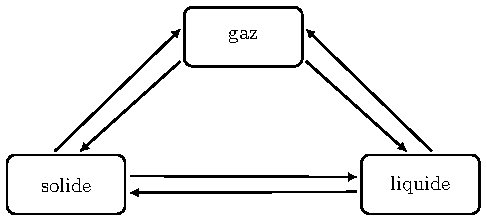
\includegraphics[width=.8\linewidth]{phases_trstion-stud}
		}{
			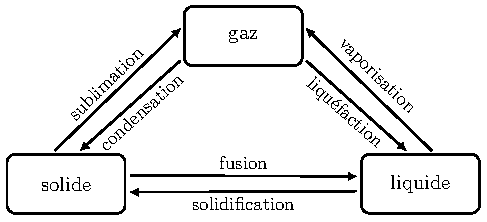
\includegraphics[width=.8\linewidth]{phases_trstion}
		}
		\captionof{figure}{Vocabulaire des transitions de phase}
	\end{center}
\end{tcb*}
Pour une animation utilisée tout au long de ce chapitre, voir \url{https://phet.colorado.edu/sims/html/states-of-matter/latest/states-of-matter_all.html}.
\begin{tcb}(rema)<lftt>{Vocabulaire des transitions de phase}
	\begin{itemize}
		\item La vaporisation regroupe deux types de transformations liquide $\ra$
		      gaz~:
		      \begin{itemize}
			      \item[b]{Ébullition}:
			      \psw{%
				      vaporisation \textbf{dans la masse}
			      }%
			      \item[b]{Évaporation}:
			      \psw{%
				      vaporisation \textbf{à la surface}
			      }%
		      \end{itemize}
		\item On appelle parfois la liquéfaction une \textbf{condensation liquide},
		      et la condensation une condensation solide.
	\end{itemize}
\end{tcb}

Dans toute la suite, on s'intéresse à un corps pur diphasé à l'équilibre~:
\begin{itemize}
	\item[b]{Corps pur}: \psw{une seule espèce chimique}
	\item[b]{Diphasé}: \psw{présente sous deux phases, par exemple liquide et gaz}
	\item[b]{À l'équilibre}: \psw{$P$ et $T$ sont les mêmes dans les deux phases}
\end{itemize}

\subsection{Diagramme $(P,T)$}
Pour chaque corps pur, on peut établir expérimentalement des diagrammes de
phases qui indiquent sous quelle phase le corps se présente suivant les valeurs
de certaines variables d’état. Le diagramme le plus simple est le diagramme
$(P,T)$~:
\begin{tcb*}(defi){Diagramme $(P,T)$}
	Un diagramme $(P,T)$ présente les \textbf{états d'un corps pur} avec la pression $P$
	en ordonnée et la température $T$ en abscisse, séparés par les \textbf{courbes
		d'équilibre diphasé}. Il y a deux cas de diagrammes $(P,T)$~:
	\smallbreak
	\begin{isd}
		\begin{center}
			\sswitch{
				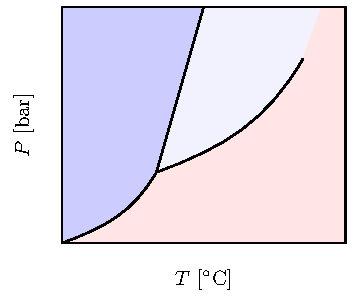
\includegraphics[width=\linewidth]{PT_gen-stud}
			}{
				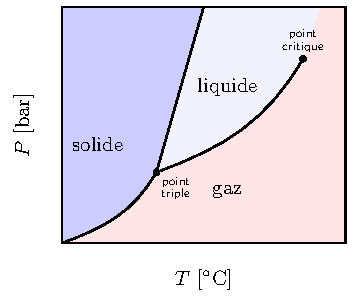
\includegraphics[width=\linewidth]{PT_gen}
			}
			\vspace{-25pt}
			\captionof{figure}{Diagramme $(P,T)$ général.}
		\end{center}
		\tcblower
		\begin{center}
			\sswitch{
				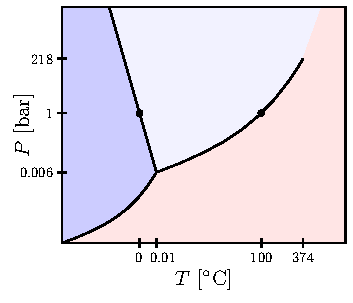
\includegraphics[width=\linewidth]{PT_eau-stud}
			}{
				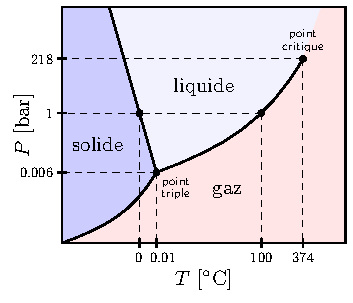
\includegraphics[width=\linewidth]{PT_eau}
			}
			\vspace{-25pt}
			\captionof{figure}{Diagramme $(P,T)$ de l'eau.}
		\end{center}
	\end{isd}
	\begin{itemize}
		% \item[b]{Courbes d'équilibre diphasé}: ce sont les courbes où \textbf{deux
		% 	phases peuvent coexister}. Elles séparent les domaines des différentes
		% phases, et sont franchies lors des transitions de phase.
		\item[b]{Point triple T}: seul point $(P\ind{T},T\ind{T})$ où il y
		a \textbf{coexistence des phases}\ftn{Voir
			\url{https://www.youtube.com/watch?v=XEbMHmDhq2I}.}.
		\item[b]{Point critique C}: point extrême de la courbe de vaporisation.
		Au-delà de ce point, les phases liquide et gazeuse ne forment plus qu'une
		phase~: on parle de \textbf{fluide supercritique}\ftn{Voir
			\url{https://www.youtube.com/watch?v=zv4sE7R8QO4} et
			\url{https://planet-terre.ens-lyon.fr/ressource/fluide-supercritique.xml}.}.
	\end{itemize}
\end{tcb*}

\begin{tcb*}(ror){Grandeurs d'état d'équilibre diphasé}
	La coexistence d'un corps pur sous deux phases à l'équilibre impose une
	dépendance de la pression avec la température~:
	\psw{%
		\[
			\boxed{P\ind{diphasé} = f (T\ind{diphasé})}
		\]
	}%
	On dit que le système est \textbf{monovariant}~:
	\begin{itemize}
		\item Pour $T$ fixée, il n'existe qu'une seule pression de coexistence~;
		\item Pour $P$ fixée, il n'existe qu'une seule température de coexistence.
	\end{itemize}
\end{tcb*}

\begin{tcb*}(defi){Pression de vapeur saturante}
	Dans le cas spécifique de l'équilibre liquide-vapeur, la pression d'équilibre
	est appelée \textbf{pression de vapeur saturante} $P\ind{sat}(T)$. Par
	exemple, pour $T$ fixée~:
	\begin{itemize}
		\item $P < P\ind{sat}(T) \Ra$
		      \psw{système sous forme de vapeur dite \textbf{sèche}~;}
		\item $P = P\ind{sat}(T) \Ra$
		      \psw{équilibre diphasé, coexistence de liquide et de vapeur dite
			      \textbf{saturante}~;}
		\item $P > P\ind{sat}(T) \Ra$
		      \psw{système sous forme de liquide uniquement.}
	\end{itemize}
\end{tcb*}

\subsection{Diagramme $(P,v)$ (de \textsc{Clapeyron})}
\subsubsection{Construction}
À la frontière d’un changement d’état sur un diagramme $(P,T)$, il y a
coexistence de deux phases, dans des \textbf{proportions différentes}. Pour
représenter l’état du système au cours du changement de phase, on utilise alors
un diagramme de \textsc{Clapeyron} $(P,v)$.
\smallbreak
On s'intéresse ici à la construction de ce diagramme par une expérience simple~:
on emprisonne un gaz dans un récipient étanche et \textbf{thermostaté} à $T_0$.
On comprime le gaz et on mesure la pression~:
\bigbreak
\noindent
\begin{tabularx}{\linewidth}{lYYYY}
	\toprule
	\textbf{État}
	 &
	\textbf{État A}
	 &
	\textbf{État B}
	 &
	\textbf{État C}
	 &
	\textbf{État D}
	\\
	\midrule
	\textbf{Schéma}
	 &
	\begin{center}
		\sswitch{
			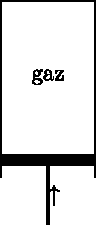
\includegraphics[width=2cm, draft=true]{Pv_constru_A}
		}{
			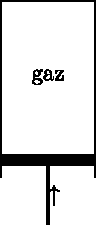
\includegraphics[width=2cm]{Pv_constru_A}
		}
	\end{center}
	 &
	\begin{center}
		\sswitch{
			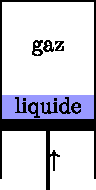
\includegraphics[width=2cm, draft=true]{Pv_constru_B}
		}{
			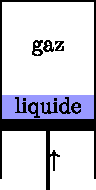
\includegraphics[width=2cm]{Pv_constru_B}
		}
	\end{center}
	 &
	\begin{center}
		\sswitch{
			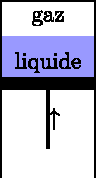
\includegraphics[width=2cm, draft=true]{Pv_constru_C}
		}{
			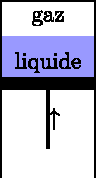
\includegraphics[width=2cm]{Pv_constru_C}
		}
	\end{center}
	 &
	\begin{center}
		\sswitch{
			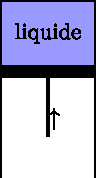
\includegraphics[width=2cm, draft=true]{Pv_constru_D}
		}{
			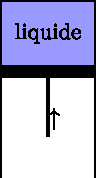
\includegraphics[width=2cm]{Pv_constru_D}
		}
	\end{center}
	\\
	\midrule
	\textbf{Composition}
	 &
	\psw{Vapeur sèche}
	 &
	\psw{Mélange liquide-vapeur}
	 &
	\psw{Mélange liquide-vapeur}
	 &
	\psw{Liquide uniquement}
	\\
	\midrule
	\textbf{Variation}
	 &
	\psw{$v \searrow$, $P \nearrow$}
	 &
	\psw{$v \searrow$, $P = \cte$}
	 &
	\psw{$v \searrow$, $P = \cte$}
	 &
	\psw{$v \searrow$, $P \nearrow\nearrow$}
	\\
	\bottomrule
\end{tabularx}

\bigbreak
On obtient alors l'évolution suivante en diagramme de \textsc{Clapeyron}~:
\smallbreak
\noindent
\begin{minipage}[t]{\linewidth}
	\begin{center}
		\sswitch{
			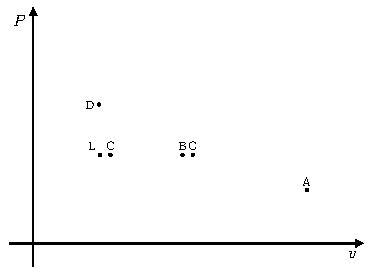
\includegraphics[width=.5\linewidth]{Pv_one-stud}
		}{
			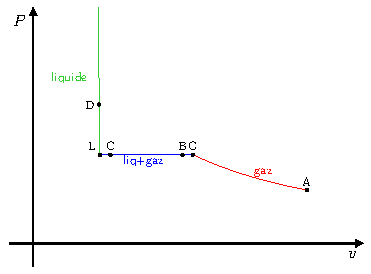
\includegraphics[width=.5\linewidth]{Pv_one}
		}
		\vspace{-15pt}
		\captionof{figure}{Isotherme d'\textsc{Andrews}}
	\end{center}
\end{minipage}

\subsubsection{Lecture}
\begin{tcb*}(defi){Diagramme $(P,v)$}
	Un diagramme $(P,v)$ représente les états d'un corps pur avec la pression $P$
	en ordonnée et le \textbf{volume massique} en abscisse, donnant accès à
	d'autres informations sur l'équilibre liquide-vapeur~:
	\begin{isd}
		\begin{itemize}
			\item[b]{Isothermes d'\textsc{Andrews}}:
			\psw{courbes d'évolution pour $T = \cte$~;}
			\item[b]{Courbe de rosée}:
			\psw{%
				frontière entre les domaines diphasé et gazeux. On y trouve la première
				goutte de liquide dans un gaz~;
			}%
			\item[b]{Courbe d'ébullition}:
			\psw{%
				frontière entre les domaines liquide et diphasé. On y trouve la première
				bulle de gaz dans un liquide~;
			}%
			\item[b]{Zone supercritique}:
			\psw{%
				pour $T \geq T_C$, le système est sous forme de fluide supercritique, il
				n'y a plus de transition liquide-gaz.
			}%
		\end{itemize}
		\tcblower
		\begin{center}
			\sswitch{
				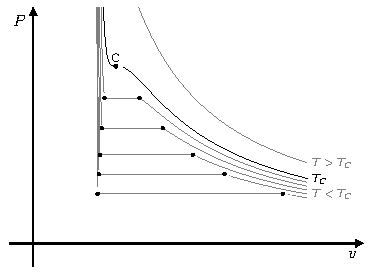
\includegraphics[width=\linewidth]{Pv_full-stud}
			}{
				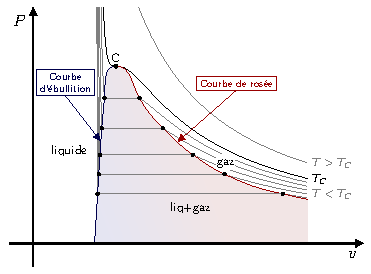
\includegraphics[width=\linewidth]{Pv_full}
			}
			\vspace{-15pt}
			\captionof{figure}{Diagramme $(P,v)$}
		\end{center}
	\end{isd}
\end{tcb*}

\begin{tcb}[sidebyside, righthand ratio=.4](rema)<lftt>{$P\ind{sat}(T)$ et combinaison des diagrammes}
	\begin{itemize}
		\item On retrouve la pression de vapeur saturante lorsqu'il y a coexistence
		      du liquide et de la vapeur.
		\item Les deux diagrammes dérivent d'une version plus complète à 3
		      dimensions, le diagramme $(P,v,T)$.
		      \begin{itemize}
			      \item Un état est un point de la surface~;
			      \item Le diagramme $(P,T)$ s'obtient en regardant selon $v$~;
			      \item Le diagramme $(P,v)$ s'obtient en regardant selon $T$, et les
			            isothermes sont obtenues par des coupes à $T = \cte$.
		      \end{itemize}
	\end{itemize}
	\tcblower
	\begin{center}
		\includegraphics[width=1\linewidth]{Pvt}
	\end{center}
\end{tcb}
\begin{tcb*}(odgr)<lftt>{Volumes massiques}
	\psw{%
		\[
			v\ind{gaz} \approx \num{1000}v\ind{liquide}
			\Lra
			\rho\ind{gaz} \approx \frac{\rho\ind{liquide}}{1000}
		\]
	}%
	\vspace{-15pt}
\end{tcb*}

\subsubsection{Théorème des moments}

\begin{tcb*}(defi){Titres massiques}
	Soit $m$ la masse totale du système diphasé, $m_{\ell}$ celle du liquide et
	$m_g$ celle de gaz. On définit les \textbf{titres massiques} en gaz et en
	liquide tels que~:
	\[
		\psw{x_g = \frac{m_g}{m_g+m_{\ell}}}
		\qqet
		\psw{x_{\ell} = \frac{m_{\ell}}{m_g+m_{\ell}}}
		\qqMath{tels que}
		\psw{x_g + x_{\ell} = 1}
	\]
\end{tcb*}

\begin{tcb*}[sidebyside, lefthand ratio=.6](prop){Théorème des moments}
	Pour un équilibre liquide-gaz à $T_0$, $P\ind{sat}(T_0)$ et pour $v = V/m$
	fixé, les titres massiques se lisent sur un diagramme $(P,v)$ tels que
	\[
		\psw{\boxed{x_{\ell} = \frac{MG}{LG} = \frac{v_g - v}{v_g-v_{\ell}}}}
		\qqet
		\psw{\boxed{x_g = \frac{ML}{LG} = \frac{v - v_{\ell}}{v_g-v_{\ell}}}}
	\]
	\tcblower
	\begin{center}
		\sswitch{
			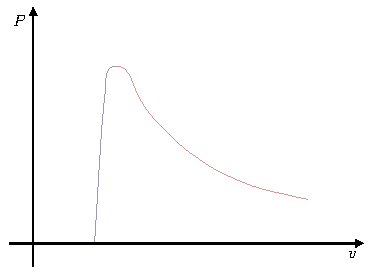
\includegraphics[width=\linewidth]{Pv_moment-stud}
		}{
			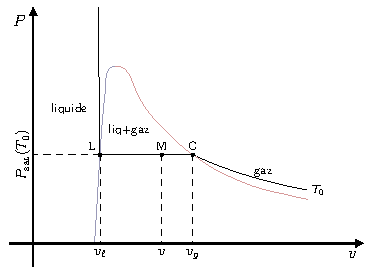
\includegraphics[width=\linewidth]{Pv_moment}
		}
		\vspace{-15pt}
	\end{center}
\end{tcb*}

\begin{tcb*}(demo){Théorème des moments}
	Soit $V_g$ et $V_{\ell}$ les volumes de gaz et de liquide, et $V = V_g +
		V_{\ell}$ le volume total.
	\psw{%
		\begin{DispWithArrows*}[]
			v &= \frac{V_g}{m} + \frac{V_{\ell}}{m}
			\Arrow{$v = V/m \Lra V = mv$}
			\\\Lra
			v &= \frac{m_gv_g}{m} + \frac{m_{\ell}v_{\ell}}{m}
			\Arrow{$x_g = m_g/m$}
			\\\Lra
			v &= x_gv_g + x_{\ell}v_{\ell}
			\Arrow{$x_g = 1-x_{\ell}$}
			\\\Lra
			v &= (1-x_{\ell})v_g + x_{\ell}v_{\ell}
			\\\Lra
			x_{\ell} = \frac{v_g-v}{v_g-v_{\ell}}
			\quad & \text{et} \quad
			x_g = \frac{v-v_{\ell}}{v_g-v_{\ell}}
			\qed
		\end{DispWithArrows*}
	}%
	\vspace{-15pt}
\end{tcb*}

\begin{tcb*}(inte){Théorème des moments}
	Ce résultat est intuitif~: il y a d'autant plus de gaz que son volume moyen
	est proche de celui de la phase gazeuse pure, c'est-à-dire que M est proche de
	G~!
\end{tcb*}

\begin{tcb}(rema)<lftt>{Théorème des moments}
	\begin{itemize}
		\item Quelle que soit la variable extensive $Y$ (enthalpie ou entropie par
		      exemple), on peut démontrer le théorème des moments avec $y$, $y_{\ell}$
		      et $y_g$.
		\item Le théorème reste valable pour les grandeurs molaires.
	\end{itemize}
\end{tcb}

\subsubsection{Bilan}
\begin{tcb*}(ror){Bilan équilibre diphasé}
	Pour connaître la composition et l'état d'un système diphasé, il suffit de
	préciser~:
	\begin{itemize}
		\item la pression \textbf{ou} la température~: en connaissant l'un, on
		      déduit l'autre par le diagramme $(P,T)$~; à $T$ connue un changement
		      d'état se fait à pression fixée et inversement~;
		\item titre massique ou le volume massique~:
		      \begin{itemize}
			      \item Le théorème des moments permet d'avoir les fractions massiques
			            à partir du volume massique~;
			      \item $v = x_gv_g + x_{\ell}v_{\ell}$ permet d'avoir le volume
			            massique à partir des fractions massiques
		      \end{itemize}
	\end{itemize}
	Pour connaître les phases en présence, on \textbf{pose une hypothèse} puis on
	\textbf{vérifie la cohérence} des résultats obtenus.
\end{tcb*}

\begin{tcb*}(appl)<lftt>{Équilibre de l'eau}
	On place une masse $m = \SI{10}{g}$ d'eau liquide dans une enceinte de volume
	$V = \SI{10}{L}$ initialement vide. Cette enceinte est maintenue à la
	température $T = \SI{373}{K}$. On donne $v_g(\SI{373}{K}) =
		\SI{1.673}{m^3.kg^{-1}}$ et $v_{\ell}(\SI{373}{K}) =
		\SI{1.04e-3}{m^3.kg^{-1}}$.
	\smallbreak
	\textbf{Calculer le volume massique moyen $v$ du système et en déduire les
		phases présentes dans l'état final ainsi que les titres en vapeur et en
		liquide}.
	\tcblower
	\begin{itemize}
		\item[b]{Volume massique moyen}:
		\vspace{-25pt}
		\psw{%
			\begin{gather*}
				v = V/m = \SI{1}{m^3.kg^{-1}}
			\end{gather*}
		}%
		\vspace{-15pt}
		\item[b]{Eau liquide pure}:
		\vspace{-25pt}
		\psw{%
			\begin{gather*}
				x_{\ell} = 1
				\Ra
				v = v_{\ell}
				\tag*{impossible}
			\end{gather*}
		}%
		\vspace{-15pt}
		\item[b]{Eau gazeuse pure}:
		\vspace{-25pt}
		\psw{%
			\begin{gather*}
				x_g = 1
				\Ra
				v = v_g
				\tag*{impossible}
			\end{gather*}
		}%
		\vspace{-15pt}
		\item[b]{Équilibre diphasé}:
		\vspace{-25pt}
		\psw{%
			\begin{gather*}
				x_g = \num{0.60}
				\qqet
				x_{\ell} = \num{0.40}
			\end{gather*}
		}%
	\end{itemize}
	\vspace{-25pt}
\end{tcb*}

\subsubsection{Application~: stockage des fluides}

Le stockage des gaz est problématique du fait de leurs faible volume massique à
pression atmosphérique et température ambiante : $v_g(\SI{300}{K}, \SI{1}{bar})
	\approx \SI{1}{m^3.kg^{-1}}$. On cherche donc à les stocker sous haute pression
pour réduire l’encombrement. Le point critique joue un rôle important dans le
choix des conditions de stockage.
\begin{itemize}
	\item[b]{$T_C < T\ind{ambiant}$}: fluide supercritique, donc quelle que soit
	la pression le système est fluide (par exemple, $T_C(\ce{O_2}) =
		\SI{155}{K}$).

	\item[b]{$T_C > T\ind{ambiant}$}: en comprimant le système, on fait apparaître
	une phase liquide en équilibre avec la phase vapeur, ce qui réduit
	l'encombrement du système ($v_{\ell} \ll v_g$) (par exemple, $T_C
		(\ce{butane}) = \SI{425}{K}$).
\end{itemize}

Cependant, en cas d'échauffement accidentel (incendie par exemple), le fluide
stocké évolue à volume massique constant le long d'une verticale sur le
diagramme de \textsc{Clapeyron}, d'une isotherme $T$ à une isotherme $T'>T$. On
distingue alors deux situations~:
\smallbreak
\begin{isd}[righthand ratio=.3]
	\begin{itemize}
		\item[b]{$v < v_C$} faible titre en vapeur, évolution MM'~;
		\item[b]{$v > v_C$} fort titre en vapeur, évolution NN'.
		\olditem[?] Pour quelle évolution le risque d'explosion de l'enceinte est-il le plus
		faible~?
		\olditem[$\Ra$]
		\psw{%
			Pour NN', on obtient du gaz et la pression est bien plus faible~: moins de
			risque d'explosion~!
		}%
	\end{itemize}
	\tcblower
	\begin{center}
		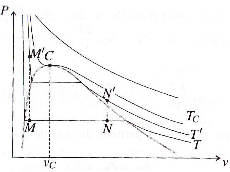
\includegraphics[width=\linewidth]{stock_eau}
	\end{center}
	% TODO: Refaire figure
\end{isd}

\begin{tcb}(impl){Stockage des fluides}
	Il est essentiel que le \textbf{volume massique du fluide stocké soit
		\xul{\psw{supérieur}} au volume massique critique $v_C$}.
\end{tcb}

\section{Thermodynamique des transitions de phase}
\subsection{Enthalpie}
Le fait de \textbf{changer l'état} d'un corps s'accompagne d'une
\textbf{variation d'énergie}. C'est d'ailleurs pourquoi le changement se fait à
température constante pour une pression fixée~: toute \textbf{l'énergie
	échangée} est utilisée pour la \textbf{réorganisation de phase} du corps pur.

\begin{tcb*}(defi){Enthalpie de changement d'état}
	Soit A et B deux phases d'un corps pur. Pour une transformation isotherme à la
	température $T$ (et donc isobare à $P = P\ind{diphasé}(T)$), l'enthalpie
	massique de changement d'état est
	\psw{%
		\[
			\boxed{\Delta{h}_{A\to B}(T) = h_B(T) - h_A(T)} = \ell_{A\to B}
		\]
	}%
	que l'on appelle également \textbf{chaleur latente} massique de transition de
	phase.
\end{tcb*}

\begin{tcb*}(exem)<lftt>{Enthalpies de changement d'état}
	Soit $h_s$, $h_{\ell}$ et $h_g$ les enthalpies massiques d'un système en phase
	solide, liquide ou gazeuse. On définit les enthalpies de changement d'état
	suivantes~:
	\smallbreak
	\begin{isd}
		\begin{itemize}
			\item
			      \leftrights{%
				      \textbf{Fusion}~:
			      }{%
				      $\psw{\Delta{h}\ind{fus} = h_{\ell} - h_s > 0}$
			      }%
			\item
			      \leftrights{%
				      \textbf{Vaporisation}~:
			      }{%
				      $\psw{\Delta{h}\ind{vap} = h_g - h_{\ell} > 0}$
			      }%
			\item
			      \leftrights{%
				      \textbf{Sublimation}~:
			      }{%
				      $\psw{\Delta{h}\ind{sub} = h_g - h_s > 0}$
			      }%
		\end{itemize}
		\tcblower
		\begin{itemize}
			\item
			      \leftrights{%
				      \textbf{Solidification}~:
			      }{%
				      $\psw{\Delta{h}\ind{sol} = -\Delta{h}\ind{fus} < 0}$
			      }%
			\item
			      \leftrights{%
				      \textbf{Liquéfaction}~:
			      }{%
				      $\psw{\Delta{h}\ind{liq} = -\Delta{h}\ind{vap} < 0}$
			      }%
			\item
			      \leftrights{%
				      \textbf{Condensation}~:
			      }{%
				      $\psw{\Delta{h}\ind{cond} = -\Delta{h}\ind{sub} < 0}$
			      }%
		\end{itemize}
	\end{isd}
	\vspace{-25pt}
\end{tcb*}

\begin{tcb*}(ror){Enthalpies de changement d'état}
	Ainsi, il faut \textbf{apporter de l'énergie} pour passer de la phase la
	\textbf{plus ordonnées} à la \textbf{moins ordonnée}~; on dit alors que la
	transition de phase est \textbf{endothermique}. À l'inverse, on
	\textit{cède de l'énergie} pour passer de la \textit{moins ordonnée} à la
	\textit{plus ordonnée}~; on la dit alors \textit{exothermique}.
\end{tcb*}

\begin{tcb*}(inte){Enthalpies de changement d'état}
	\begin{center}
		\sswitch{
			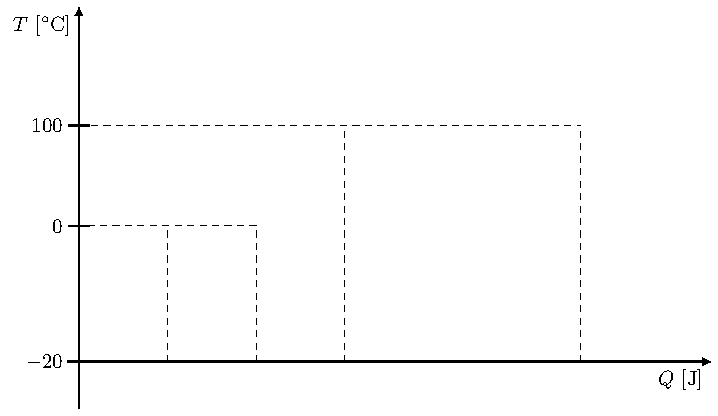
\includegraphics[width=.8\linewidth]{TQ_eau-stud}
		}{
			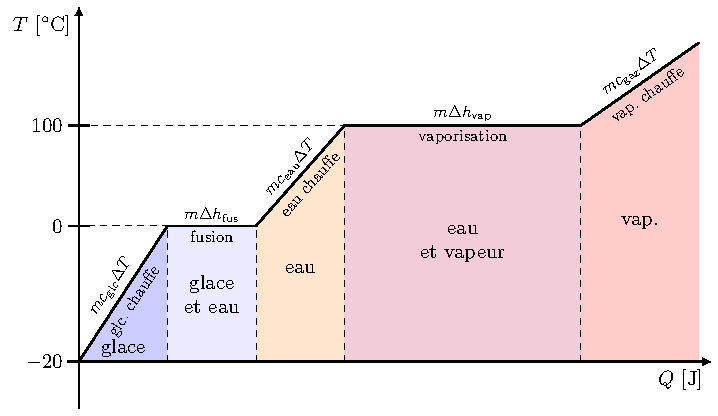
\includegraphics[width=.8\linewidth]{TQ_eau}
		}
		\vspace{-15pt}
		\captionof{figure}{Augmentation de la température de l'eau en fonction de
			l'énergie apportée.}
	\end{center}
\end{tcb*}

\begin{tcb*}(odgr)<lftt>{Enthalpies de changement d'état}
	\begin{tasks}[label=\bdmd](2)
		\task $\Delta{h}\ind{fus} = \SI{330}{kJ.kg^{-1}}$
		\task $\Delta{h}\ind{vap} = \SI{2.26}{MJ.kg^{-1}}$
	\end{tasks}
	Il faut donc \textbf{bien plus d'énergie} pour \textbf{changer de phase} que
	pour \textbf{chauffer une phase} ($c\ind{eau,liq} = \SI{4.18}{kJ.kg^{-1}}$).
\end{tcb*}

\begin{tcb*}(ror){Détermination état final diphasé}
	\begin{enumerate}[label=\sqenumi]
		\item[b]{Hypothèse}: soit le système est monophasé, soit diphasé.
		\begin{itemize}
			\item[b]{Si monophasé}: on cherche $T_f$ en prenant en compte le
			changement de phase.
			\item[b]{Si diphasé}: on exprime la masse ayant changé d'état (à tester
			entre phase A et phase B), sachant que l'\textbf{équilibre} n'est
			possible qu'à la \textbf{température de changement d'état}.
		\end{itemize}
		\item[b]{Calcul}: on utilise l'additivité de l'enthalpie~: $\Delta{H} =
			\Delta{H}_A + \Delta{H}_B$, en prenant en compte le changement de
		température \textbf{et} le changement de phase.
		\item[b]{Vérification}: on vérifie que le résultat soit cohérent. S'il ne
		l'est pas (par exemple, eau gazeuse à \SI{300}{K} et $\SI{1}{bar}$
		impossible), on change l'hypothèse de base et on recommence.
	\end{enumerate}
\end{tcb*}

\begin{tcb*}(appl)<lftt>{Calorimétrie avec changement d'état}
	On place $m_0 = \SI{40}{g}$ de glaçons à $T_0 = \SI{0}{\degreeCelsius}$ dans
	$m_1 = \SI{300}{g}$ d'eau à $T_1 = \SI{20}{\degreeCelsius}$ à l'intérieur
	d'un calorimètre de capacité $C = \SI{150}{J.K^{-1}}$. Déterminer la
	température d'équilibre $T_f$, sachant que $c\ind{eau} =
		\SI{4185}{J.K^{-1}.kg^{-1}}$ et $\Delta{h}\ind{fus} = \SI{330}{kJ.kg^{-1}}$.
	\tcblower
	\vspace{-15pt}
	\psw{%
		\begin{align*}
			\beforetext{Calorimètre}
			\Delta{H}\ind{calo}  & = C (T_f-T_1)
			\tag*{}
			\\\beforetext{Eau liquide}
			\Delta{H}\ind{eau}   & = m_1c\ind{eau}(T_f-T_1)
			\tag*{\textbf{hypothèse}}
			\\\beforetext{Glace}
			\Delta{H}\ind{glace} & = m_g (h_{\ell}(T_f) - h_g (T_0))
			\\\Lra
			\Delta{H}\ind{glace} & =
			m_g \big(
			\underbracket[1pt]{h_{\ell}(T_f) - h_{\ell}(T_0)}_{c\ind{eau}(T_f-T_0)} +
			\underbracket[1pt]{h_{\ell}(T_0) - h_g (T_0)}_{\Delta{h}\ind{fus}}
			\big)
			\\\beforetext{Additivité}
			\Ra
			\Delta{H}            & =
			\Delta{H}\ind{calo} + \Delta{H}\ind{eau} + \Delta{H}\ind{glace}
			\\\beforetext{Isobare et isolé}
			\Delta{H}            & = Q = 0
			\\\Lra
			0                    & =
			(C + m_1c\ind{eau}) (T_f - T_1) +
			m_g\Delta{h}\ind{fus} +
			m_gc\ind{eau} (T_f - T_0)
			\\\Lra
			\Aboxed{
			T_f                  & =
				\frac{
					(C + m_1c\ind{eau}) T_1 + m_gc\ind{eau} T_0 - m_g\Delta{h}\ind{fus}
				}{
					C + m_1c\ind{eau} + m_gc\ind{eau}
				}
			}
			\\
			\makebox[0pt][l]{$\phantom{\AN}\xul{\phantom{T_f = \SI{9.5}{\degreeCelsius}}}$}
			\AN
			T_f                  & = \SI{9.5}{\degreeCelsius}
		\end{align*}
	}%
	\vspace{-25pt}
\end{tcb*}

\vspace{-20pt}
\subsection{Entropie}
Avec le paragraphe précédent, il est donc évident que changer de phase
s'accompagne d'une variation d'entropie, puisque le désordre augmente. On a
ainsi~:
\begin{tcb*}(prop){Entropie de changement d'état}
	Soit A et B deux phases d'un corps pur. Pour une transformation isotherme à la
	température $T$ (et donc isobare à $P = P\ind{diphasé}(T)$), la
	\textbf{transition de phase est réversible} et l'entropie
	massique de changement d'état est
	\psw{%
		\[
			\boxed{\Delta{s}_{A\to B} = \frac{\Delta{h}_{A\to B}}{T}}
		\]
	}%
	\vspace{-15pt}
\end{tcb*}

\begin{tcb*}(demo){Entropie de changement d'état}
	Un changement d'état est réversible puisqu'il peut toujours être fait dans le
	sens inverse et est en équilibre permanent. Ainsi,
	\psw{%
		\begin{DispWithArrows*}[]
			\Delta{S} &= S\ind{ech} + \underbracket[1pt]{S\ind{cr}}_{=0}
			\Arrow{monotherme}
			\\\Lra
			\Delta{S} &= \frac{Q}{T}
			\Arrow{isobare $\Delta{H} = Q$}
			\\\Lra
			\Delta{S} &= \frac{\Delta{H}}{T}
			\Arrow{$\Delta{H} = m\Delta{h}_{1\to B}$\\$\Delta{S} = m\Delta{s}_{1\to B}$}
			\\\Lra
			\Aboxed{
				\Delta{s}_{A\to B} &= \frac{\Delta{h}_{A\to B}}{T}
			}
		\end{DispWithArrows*}
	}%
	\vspace{-15pt}
\end{tcb*}

\begin{tcb}(rema)<lftt>{Entropie de changement d'état}
	On a alors $\Delta{h}$ du même signe que $\Delta{s}$, ce qui explique
	lesquelles sont positives et lesquelles sont négatives étant donné
	l'augmentation du désordre.
\end{tcb}

\begin{tcb*}(appl)<lftt>{Entropie de changement d'état}
	Calculer l'entropie créée lors de la transformation de l'application
	précédente.
	\tcblower
	\vspace{-15pt}
	\psw{%
		\begin{align*}
			\beforetext{Calorimètre}
			\Delta{H}\ind{calo}  & = C \ln \frac{T_f}{T_1}
			\tag*{}
			\\\beforetext{Eau liquide}
			\Delta{S}\ind{eau}   & = m_1c\ind{eau} \ln \frac{T_f}{T_1}
			\\\beforetext{Glace}
			\Delta{S}\ind{glace} & = m_g (s_{\ell}(T_f) - s_g (T_0))
			\\\Lra
			\Delta{H}\ind{glace} & =
			m_g \big(
			\underbracket[1pt]{s_{\ell}(T_f) - s_{\ell}(T_0)}_{m_gc\ind{eau}\ln
					\frac{T_f}{T_0}} +
			\underbracket[1pt]{s_{\ell}(T_0) - s_g (T_0)}_{m_g
					\frac{\Delta{h}\ind{fus}}{T_0}}
			\big)
			\\\beforetext{Additivité}
			\Ra
			\Delta{S}            & =
			\Delta{S}\ind{calo} + \Delta{S}\ind{eau} + \Delta{S}\ind{glace}
			\\\beforetext{Isolé}
			\Delta{S}            & = \underbracket[1pt]{S\ind{ech}}_{=0} + S\ind{cr}
			\\\Ra
			\makebox[0pt][l]{$\phantom{\AN}\xul{\phantom{S\ind{cr} = \SI{2.67}{J.K^{-1}}}}$}
			\AN
			S\ind{cr}            & = \SI{2.67}{J.K^{-1}}
		\end{align*}
	}%
	\vspace{-25pt}
\end{tcb*}

\section{Application aux machines thermiques}
\subsection{Intérêt}

Beaucoup de machines exploitent la transition de phase liquide-vapeur d'un
fluide, puisqu'elle permet d'emmagasiner ou de fournir des énergies très
importantes à partir de faibles variations des variables d'état, tout en
conservant les avantages des liquides et des gaz~:
\begin{itemize}
	\item Les liquides ont une \textbf{grande capacité thermique} massique, mais
	      une \textbf{faible compressibilité}~: adaptés aux transferts
	      \textbf{thermiques} par contact~;
	\item Les gaz ont une \textbf{faible capacité thermique} massique, mais une
	      \textbf{grande compressibilité}~: adaptés aux transferts sous forme de
	      \textbf{travail}.
\end{itemize}
Par exemple, un des fluides réfrigérants les plus utilisés est le
R134a\ftn{1,1,1,2-tétrafluoroéthane}~: il est tel que $\Delta{h}\ind{vap} =
	\SI{215}{kJ.kg^{-1}}$ alors que $c\ind{liq} = \SI{1.4}{kJ.kg^{-1}.K^{-1}}$~:
\textbf{vaporiser \SI{1}{kg} demande la même énergie que de chauffer de
	\SI{150}{K}}.

\subsection{Réfrigérateur}
\begin{tcb}(defi){Éléments d'une machine frigorifique}
	\begin{isd}
		\begin{enumerate}
			\item[b]{Compresseur}: le fluide y \textbf{reçoit rapidement du
				travail}, ce qui \textbf{augmente sa pression et sa température}
			(transformation adiabatique)~;

			\item[b]{Condenseur/échangeur}: circuit de transfert de la chaleur à
			la source chaude ($Q_C < 0$);
		\end{enumerate}
		\tcblower
		\begin{enumerate}[start=3]
			\item[b]{Détendeur}: le fluide y \textbf{perd en pression} et en
			température, jusqu'à $T < T_F$~;

			\item[b]{Évaporateur}: le fluide frigorigène s'y évapore et
			\textbf{prélève de l'énergie} à la source froide ($Q_F > 0$).
		\end{enumerate}
	\end{isd}
	\begin{isd}
		\begin{center}
			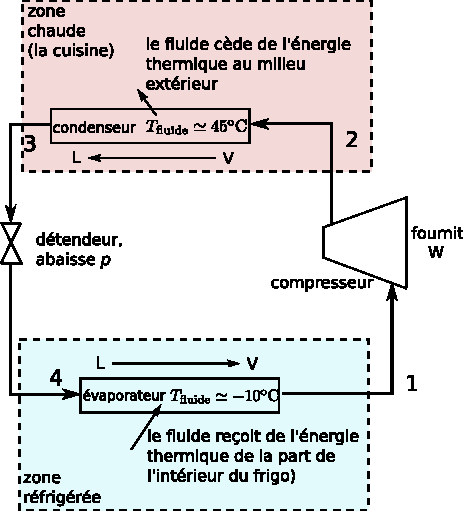
\includegraphics[width=.8\linewidth]{frigo_schema}
		\end{center}
		\tcblower
		\begin{center}
			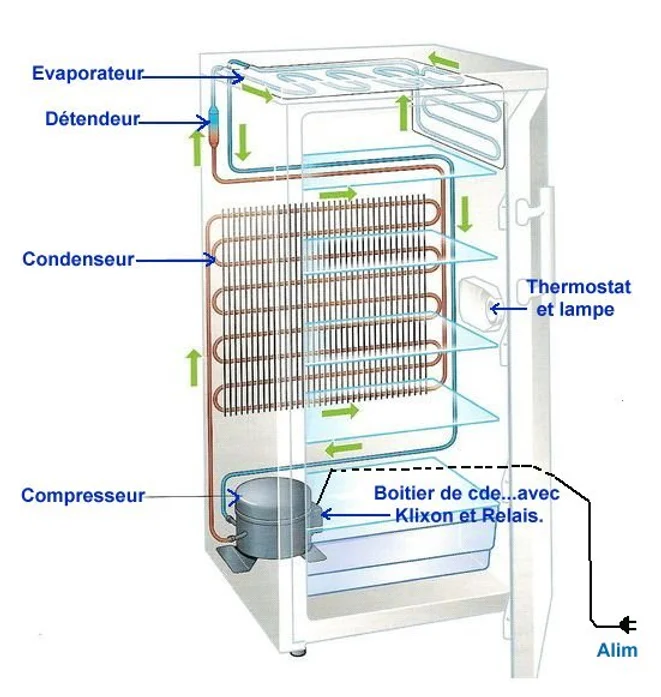
\includegraphics[width=.9\linewidth]{frigo_schema_reel-2}
		\end{center}
	\end{isd}
\end{tcb}
\subsection{Pompe à chaleur}
\begin{tcb}(exem)<lftt>{Pompe à chaleur}
	\begin{center}
		\includegraphics[scale=.9]{PAC_schema}
	\end{center}
\end{tcb}
\vspace{-15pt}
\end{document}
